\documentclass{article}
\usepackage[a4paper, margin=2cm]{geometry}
\usepackage{setspace}
%\setstretch{1.4}
\usepackage{relsize}
\usepackage{amsmath}
\usepackage{caption}
\usepackage{subcaption}
\usepackage{graphicx}
\usepackage{listings}
\usepackage{url}

\lstset{
  basicstyle=\ttfamily,
  columns=fullflexible,
}

\title{Assignment 3: Real-Time Implementation of 2D
Digital Waveguide\\
[0.2em]\smaller{ECS7012P Music and Audio Programming}}
\author{Andrea Martelloni}

\date{\today}

\begin{document}

\maketitle


\section{Introduction}

A specific class of digital musical instruments, or DMI, aims to
decouple the human playing interaction and the physical response
of the acoustic body. The instrument is thereby seen as a mute
controller interface to a digital sound-producing device.
This design paradigm allows the control of virtual instruments
based on physical models. It might be seen as bizarre to choose to
cut off the physics of an instrument, only to then try and
reproduce them as accurately as the technology allows. However,
the designer can then alter or augment the physics of the
instrument arbitrarily; for example, they could map a drum
or a set of percussions onto a guitar's body.

The work presented in this report aims to cover the first steps
in the design of such an instrument. We are going to try and
run a virtual vibrating membrane on Bela, and control it with
the signal coming from one axis of an accelerometer.

The major challenge of this task is to
ensure a correct implementation of the membrane's equations,
a requirement that can prove very tricky when programming on
an embedded target as a black box. Therefore, most of our analysis
will be performed in simulation on standard C++ code; on-target
evaluation will be the last step, a rather ambitious moment
of truth at the end of the development efforts.

\section{Background}

\subsection{Prior Work}

The numerical reproduction of percussion instruments has been
extensively studied, all the way to advanced techniques
modelling the non-linearities of such systems. Good surveys of
all available techniques come from the works by
Rossing \emph{et al.} \cite{rossing2004acoustics},
Bilbao \cite{bilbao2009modular}
and Mehes \emph{et al} \cite{mehes2017virtual}.

Implementations of purely linear model are both less computationally
intensive and easier to understand and implement. Two methods
seem to have been quite successful in reproducing membranes in
real time and are featured in working implementations of musical
instruments: the Digital Waveguide model by Fontana and Rocchesso
\cite{fontana1998physical} and the Transfer Function methods
analysed in Trautmann \emph{et al.} \cite{trautmann2001physical}.

The two-dimensional Digital Waveguide model is a well-established
model that extends the principle of the Digital Waveguide,
widely used to model tubes such as wind instruments, to a vibrating
surface.
The article referenced above provides a clear breakdown
of all the continuous-time and discrete-time physics involved,
and it provides solutions to problems such as mesh stability,
mesh excitation, energy attenuation and modelling of air loading
for a more accurate real-world drum reproduction.
Thererfore, we chose to base the implementation of our project upon
the Digital Waveguide method.

A reference implementation of a Digital Waveguide mesh is already
available in an early version
(0.62)\footnote{
\url{http://www.soundobject.org/SDT/downloads/SDT_src-062.zip}}
of the Sound Design Toolkit \cite{baldan2017sound}.
The topology of the mesh available in the toolkit is rectilinear;
however the authors describe how using a triangular mesh
optimises the dispersion error for most geometries, and especially
for the circular membranes of drums \cite{fontana1998physical}.
We will implement a triangular mesh
from first principles following this
suggestion. 

\subsection{Theory}

% Outline sources
The following summary of the theory behind digital waveguides in
a triangular mesh structure is based on \cite{fontana1998physical};
some ideas and concepts are taken from the implementation of
triangular membranes for room acoustics in \cite{murphy2000digital}.
A more complete review of the whole process applied to virtual drums
can also be found in \cite{laird2001physical}.

% Waveguide basics
\paragraph{Waveguide basics.}
The principle of the one-dimensional waveguide comes from the well-known
D'Alembert solution of the
wave wave equation for the transverse velocity \(v(t, x)\),
indicating two velocity waves travelling in opposite
directions:

\begin{equation}
v(t, x) = v_{+}(x - ct) + v_{-}(x + ct)
\end{equation}\label{eq:dalembert}

We can assume that waves propagate following the equation above
in ideal strings. When a number \(N\) of
identical strings is joined
together, we can write an equation for the transmission and
scattering of the waves among those strings at their junction
point \(i\):

\begin{equation}
v_{i-}(t) = \frac{2}{N}\,\sum_{k=1}^{N}v_{k+}(t)-v_{i+}(t)
\end{equation}\label{eq:losslessj}

\(v_{i-}\) being the outgoing wave from the junction, as a
function of the incoming waves \(v_{k+}\) from the strings
joined together.

Both equations can be discretised by sampling the space
into \(\Delta s\) spatial samples and time as \(t = nT\)
periods:

\begin{equation}
    v(nT, x) = v_{+}(x - cnT) + v_{-}(x + cnT)
\end{equation}\label{eq:discretewave}
\begin{equation}
    v_{i-}(nT) = \frac{2}{N}\,\sum_{k=1}^{N}v_{k+}(nT)-v_{i+}(nT)
\end{equation}\label{eq:discretelosslessj}

We are going to assume that the mesh is perfectly homogeneous
(no difference in impedance in the interfaces) and the boundaries
are perfectly rigid, that is, the wave is fully reflected back
(\(r = 1\))
and any point beyond the boundary will have (\(v = 0\)).

% Triangular mesh equations

\paragraph{Triangular mesh.}

Joining six waveguides we have a structure that can effectively
sample a two-dimensional space along directions \(x\),
\(l = \frac{1}{2} x + \frac{\sqrt{3}}{2} y\) and
\(m = \frac{1}{2} x - \frac{\sqrt{3}}{2} y\). Figure
\ref{fig:coord} depicts this structure and the related coordinates.

\begin{figure}
    \centering
    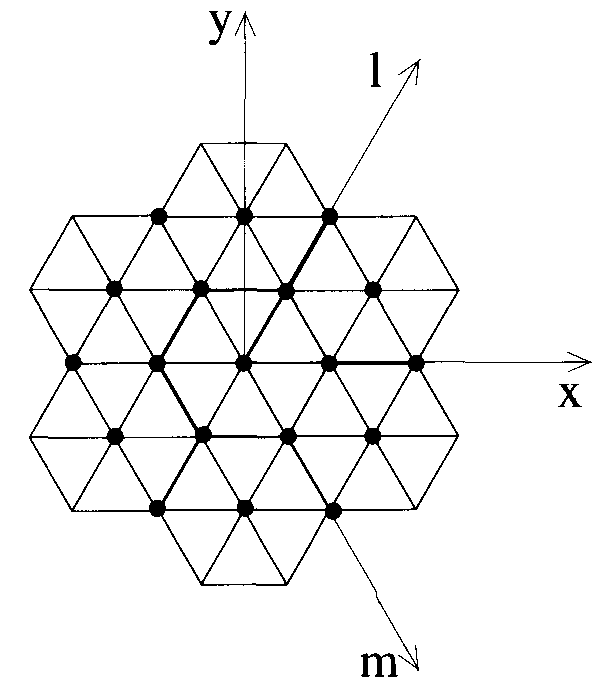
\includegraphics[width=0.4\textwidth]{fig/fontanamesh}
    \caption{Triangular mesh coordinates \cite{fontana1998physical}.}\label{fig:coord}
\end{figure}

We can then rewrite equation \ref{eq:discretelosslessj} in two
parts and restrict the number of waveguides to a maximum of 6,
assuming impedance is either homogeneous or infinite (no transmission).
We can then divide the computation into a \emph{scattering equation}
and a \emph{junction output} (after \cite{murphy2000digital}):

\begin{equation}\label{eq:scatter}
    v_{i}(nT) = \frac{2}{N}\,\sum_{k=1}^{N}v_{k+}(nT)
\end{equation}

\begin{equation}\label{eq:output}
    v_{k-}(nT) = v_{i}(nT) - v_{k+}(nT) \,\,\,\,\, \mbox{for}\, k = {1 \dots N}
\end{equation}

Junctions having fewer than six waveguides will just ignore
the directions that aren't connected to another junction point.
A good convention to enumerate the coordinates of the junction
points comes from \cite{murphy2000digital}. We will count clockwise
from the first point at top-right: North-East, East, South-East,
South-West, West and North-West.

% Courant condition

\paragraph{Constraints.}
The digital waveguide method imposes a relationship between spatial
and temporal sampling. When designing the mesh or even running
an offline simulation, one can leave the speed of the medium
\(c\) unspecified. However, in a real-time system, the temporal
sampling period \(T\) is defined by the system, and so must be the
medium speed. The stability of the mesh is enforced by the
Courant condition, which in this case takes the following
form \cite{fontana1998physical}:

\begin{equation}
\Delta x = \Delta l = \Delta m = \sqrt{2}cT
\end{equation}\label{eq:courant}

% Absorption, air loading

\paragraph{Absorption, air loading, excitation.}
The sources referenced provide a good breakdown of all the more
advanced problems around lossy junctions, air loading in
a cylindrical drum as a spring-mass model, excitation models.
We will limit ourselves to the simplest case of a lossless
stable membrane, excited directly with an arbitrary audio signal
\(y(nT)\), using the excitation model outlined
in \cite{murphy2000digital}. The source signal is injected as incoming
waves into a designated junction:

\begin{equation}\label{eq:inject}
    v_{k+}(nT) = \frac{y(nT)}{2}
\end{equation}

\section{Design}

The equations laid out in the previous section allow, in principle,
the numerical implementation of any kind of topology. However,
in addition to the memory constraints and computational constraints
imposed by the Bela target, the triangular mesh poses non-obvious
problems down to the memory layout and the change in coordinates
between cartesian and \((x, l, m)\).

The first stage of the implementation, in practice, requires
access to tools such as off-line processing,
debugging, plotting and the generation of mathematically complex
audio test signals. We found especially important to be able to
visualise the mesh at every iteration in a simulation.
For this reason, most of the code has been written within an
environment comprised of some C++ core classes, a C++ to Python
wrapper based on
Boost.Python\footnote{
    This has been the theme of a past AIL workshop at QMUL, the
    slides for which can be found here:
    \url{https://docs.google.com/presentation/d/1FK514Me0esJG-2egqraF3FT9DIQkZYGH_I2nMmFxUXI}
}
and a set of validation notebooks
written in Jupyter.

\subsection{Mesh Topology}

% Mapping meshes onto memory
Rectilinear grids have an obvious mapping onto two-dimensional arrays,
natively supported in most programming language. More complicated
topologies require a function that maps a C++ array structure to
the mesh's geometry coordinates, which we will call \(c, k\).
The idea of using a flattened array structure, albeit valid
and quite well-established, came to mind a bit too late in
the development.

\begin{figure}
    \centering
    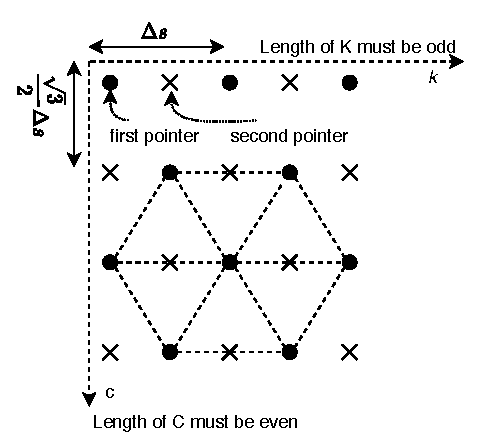
\includegraphics[width=0.4\textwidth]{fig/XYtoCK}
    \caption{Mapping between two interleaved meshes and 2D array.}\label{fig:meshmap}
\end{figure}

We present a method that maps a regular C-style 2D array structure
to a rectangular mesh topology, seen in figure \ref{fig:meshmap}.
If we impose the constraints that the column dimension of a matrix
must be even, and the rows must be odd, we can interleave two meshes
of identical size in the even and odd indexes of this matrix, respectively.
Even rows will have an odd number of mesh points, whereas odd rows
will have an even number of them. What makes this structure work
is that the third element of the second mesh in even rows is
wrapped around to the next line, therefore the indexing stays
within the required memory boundary.

The following set of equations can be used to convert back and forth
from \(c, k\) indexing and Cartesian coordinates:

\begin{equation}
    c = \frac{y}{\frac{\sqrt{3}}{2} \Delta s}
\end{equation}
\begin{equation}
    y = c\,\frac{\sqrt{3}}{2} \Delta s
\end{equation}
\begin{equation}
    k = \frac{x - \frac{\Delta s}{2} (c\,\mbox{mod}\,2)}{\Delta s}
\end{equation}
\begin{equation}
    x = k\,\Delta s + \frac{\Delta s}{2} (c\,\mbox{mod}\,2)
\end{equation}

% Mapping geometries onto meshes
Using this coordinate system, we can then assess whether each point
in the mesh lies inside or outside any geometry defined in
Cartesian coordinates. We can then choose to create a waveguide
between two points if both of them lie within the given geometry.
An example made whilst evaluating our mesh in the Jupyter notebook
is shown in figure \ref{fig:jupytermesh}.

\begin{figure}
    \centering
    \begin{subfigure}{.5\textwidth}
      \centering
      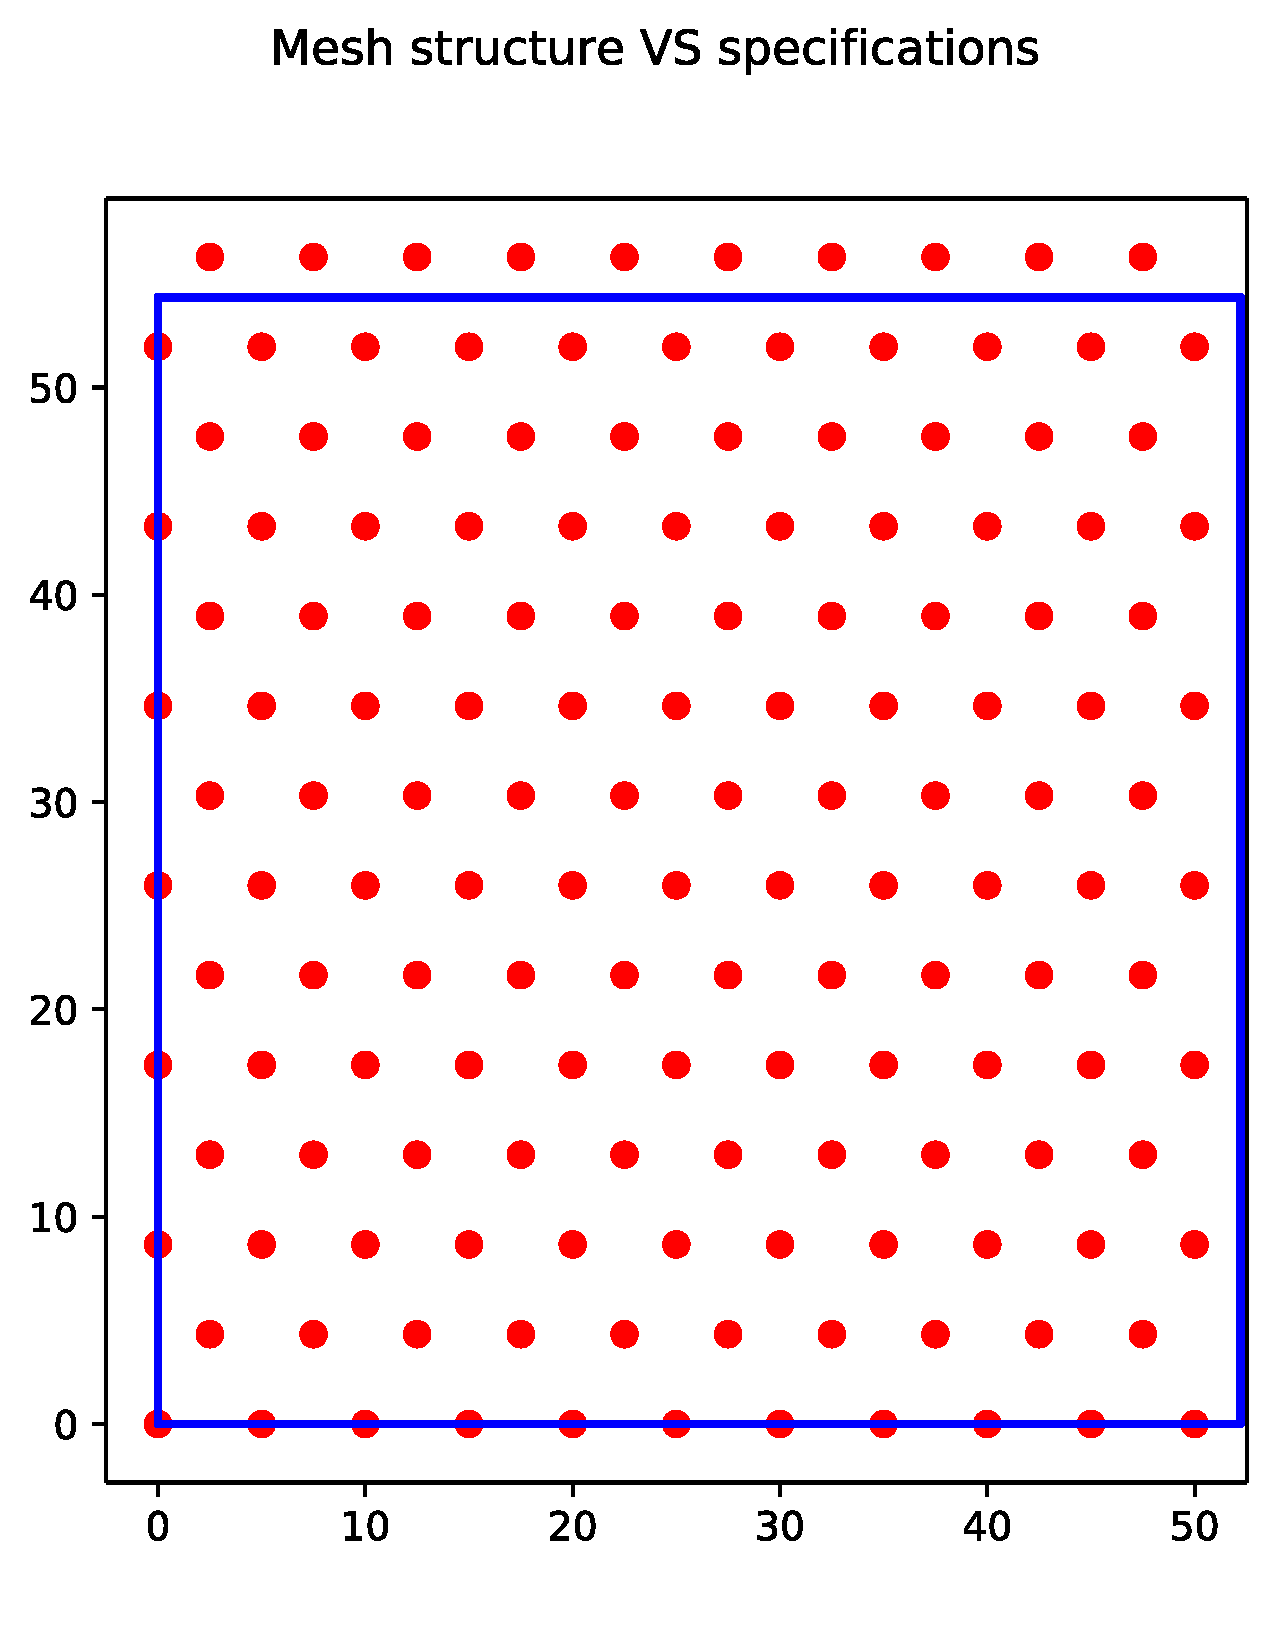
\includegraphics[width=.6\linewidth]{fig/meshsquare}
      \caption{Dimensions of the grid VS required geometry.}
      \label{fig:meshsquare}
    \end{subfigure}%
    \begin{subfigure}{.5\textwidth}
      \centering
      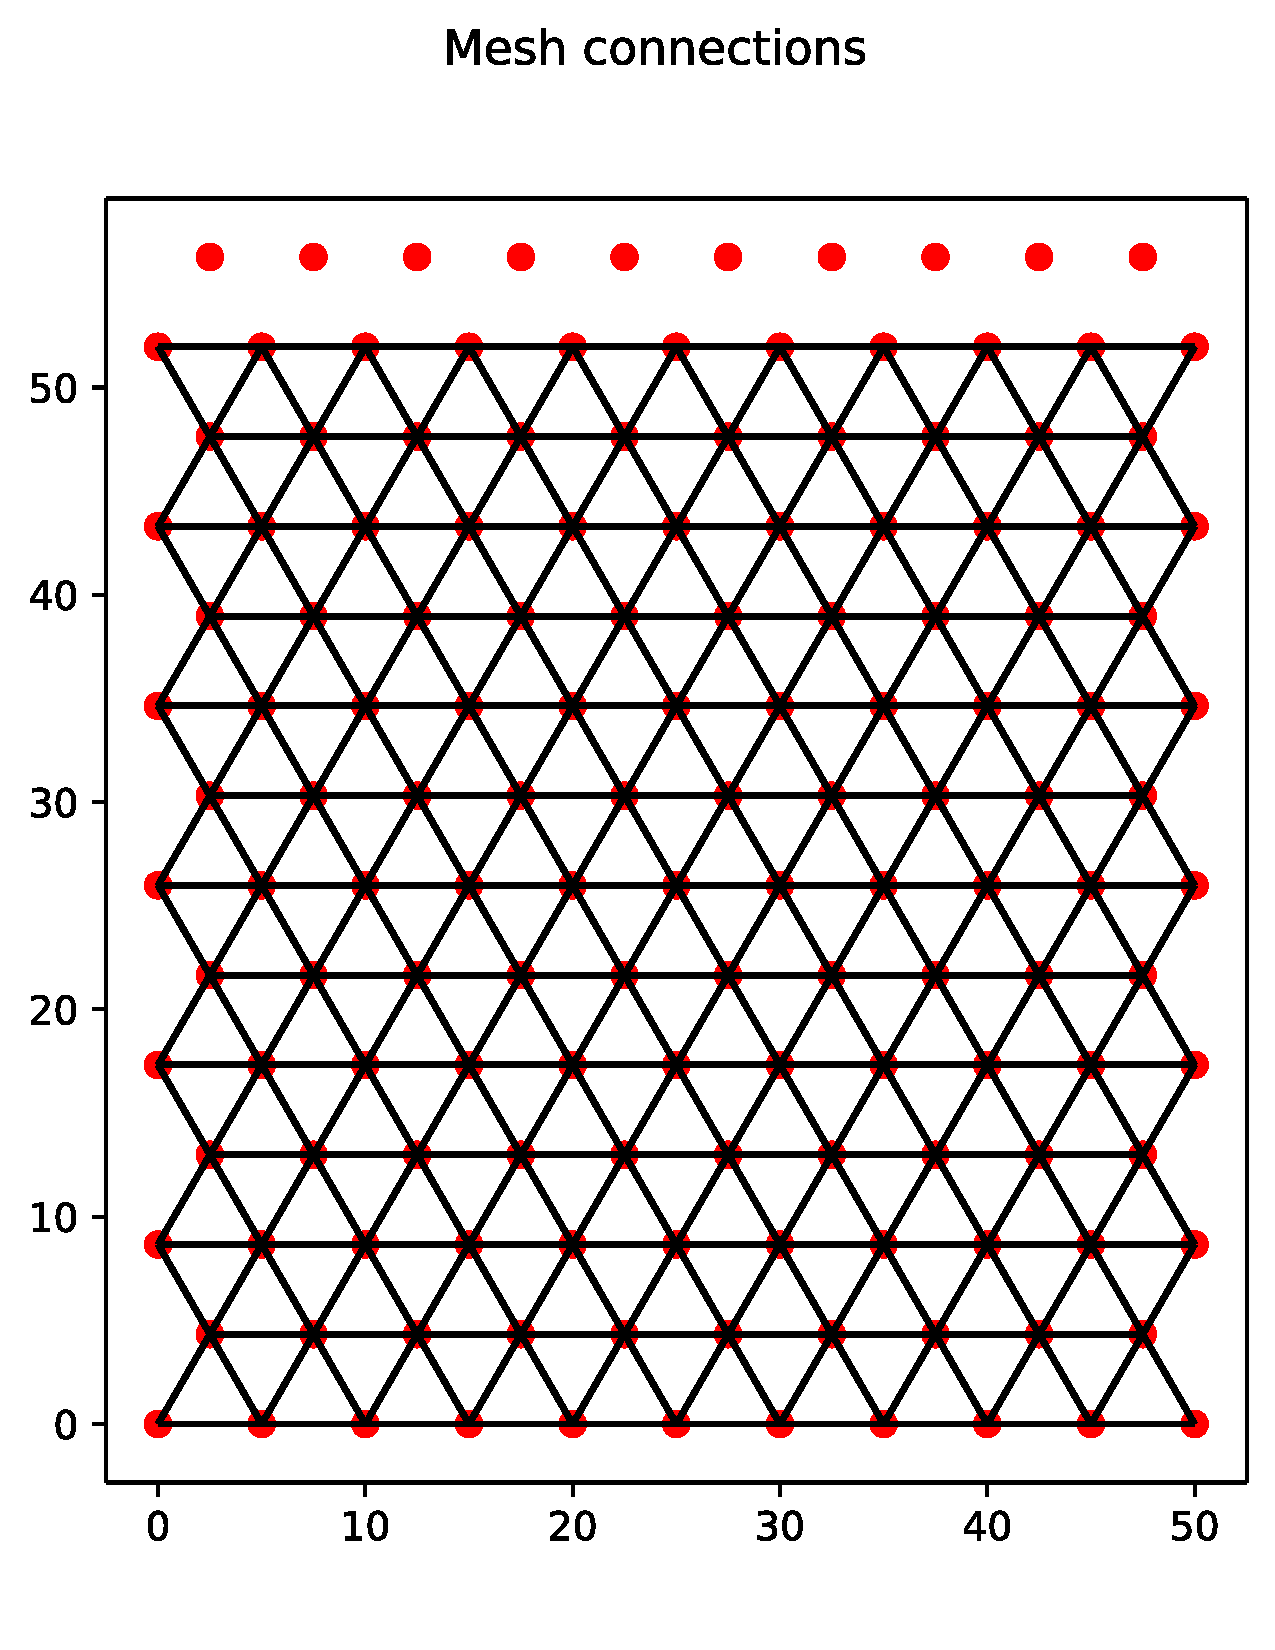
\includegraphics[width=.6\linewidth]{fig/meshgrid}
      \caption{Computed mesh connections.}
      \label{fig:meshgrid}
    \end{subfigure}
    \caption{Generated mesh for a rectangle of
    width 52.21 mm, height 54.35 mm, spatial resolution 5 mm.}
    \label{fig:jupytermesh}
\end{figure}
    

\subsection{Processing}

% Memory model for incoming V and outgoing V
The last step needed before implementing the processing routine is
to calculate how many values we need to store for each mesh point
and/or for each waveguide. Following the reference implementation in
the Sound Design Toolkit \cite{baldan2017sound}, we are going to
use two values for each waveguide, respectively an outgoing and an
incoming velocity value. The outgoing value
will be reused as an incoming value in the following time iteration
(delay step). Therefore we need a total of 13 meshes for each
mesh point, one for each waveguide plus a record of the junction
values that is going to be used for plotting.

% Junctions as bitmask
A fourteenth mesh is going to be created to store a bitmask
containing the connections between a given point and its
neighbouring point. We're going to observe Murphy's convention
of clockwise numbering from NE to NW.

Finally, we need to choose a source and a pickup point.
At startup, the source is allocated at the centre of the
membrane, whereas the pickup lies close to the edge of
the default rectangular structure, as no mode is supposed to have
a node at the corners of a shoebox shape.

All these actions are implemented in the constructor for the object
\texttt{Triangular2DMesh}: it also provides a method to externally
allocate the memory required, which is then passed as an argument
to the constructor.

Optionally, the API allows to re-draw the mesh connections based
upon a user-defined lambda expression evaluating the \(x, y\)
coordinates of each mesh point. Source an pickup points can also
be moved before or during processing.

% Translate the wave equation: each step
\texttt{ProcessSample()} implements equations
\ref{eq:scatter}, \ref{eq:output} and \ref{eq:inject} for
every point \(c, k\) in the mesh and swaps the two mesh pointers
for each iteration. The outgoing values are therefore consumed
by the neighbouring points of each junction.

\subsection{Evaluation Framework}

The simulation environment is based on an Ubuntu 20.04
Docker container. This allows the C++ and the Python bindings
to be built in a reliable environment without installing
a development toolkit system-wide.

The Bash script \texttt{docker\_host\_run.sh} will build, create
and run the appropriate Docker container; an SSH port is created
so that a remote debug session can be created via \texttt{gdb}.
The source code is automatically mounted into the Docker container's
file system, therefore any change will be picked up by both the
host machine and the container.

The Makefile supports target \texttt{test} to build a pure C++
unit test suite based on
Catch2\footnote{\url{https://github.com/catchorg/Catch2}},
and a \texttt{python} target building a shared library
\texttt{DSPPythonWrapper.so} that can be \texttt{import}ed
onto Python, and will be the basis for our validation in
Jupyter.

% Commands to run everything

\section{Bela Implementation}

The \texttt{Triangular2DMesh} object has been embedded into
a Bela project that interfaces with the same hardware prototype
built for the drum machine in Assignment 2. The accelerometer
has been reused as a transducer for low-frequency, rumble-like
displacements that are characteristic of percussive interaction.
Only the Z-axis (up-down) acceleration is needed.

Firstly, the signal from the accelerometer has been observed
from Bela's internal oscilloscope when the board was lying
on a desk, and someone was tapping on the same desk next
to the board. The resulting signal was well above the noise
floor and a clean impulse was clearly detectable.

Minimal signal conditioning has been implemented
in the \texttt{DetectHit} class: a high-pass
filter brings the accelerometer signal's mean to 0, then full-wave rectification
and a low-pass filter create a positive impulse that would inject
a controlled amount of energy onto the mesh.

\section{Evaluation}

\subsection{Unit Tests}

\texttt{make test} builds a set of unit tests implemented in
\texttt{main.cpp}: the purpose of those tests is to verify
the correct allocation of memory and the correct implementation
of the indexing routines. It is easier to debug and inspect
the routines in a pure C++ environment: a short Gaussian impulse
is passed to the processing function to ensure that the
processing happens within the memory bounds and the mesh
does not become unstable and return \texttt{Inf} or \texttt{NaN}.

This is a really limited evaluation and it does not allow
the physical validation of the formulae's implementation;
two evaluation cases have been run in a Jupyter notebook to
visualise the junction's pressure and analyse the resulting
plots.

\subsection{Simulation}

\begin{figure}
    \centering
    \begin{subfigure}{.3\textwidth}
      \centering
      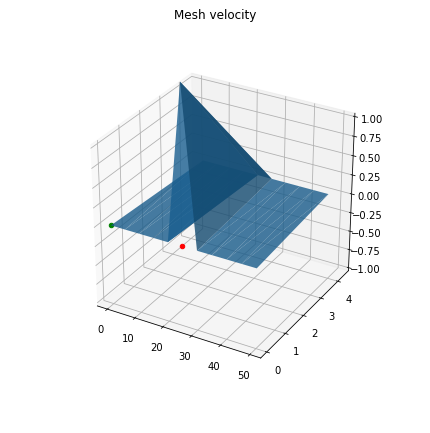
\includegraphics[width=1\linewidth]{fig/1d-sample0}
      \caption{After 1 sample.}
      \label{fig:1d-sample0}
    \end{subfigure}%
    \begin{subfigure}{.3\textwidth}
      \centering
      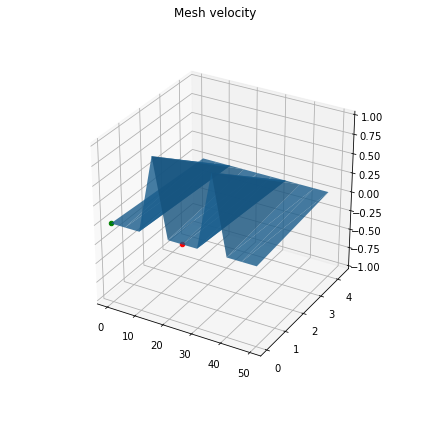
\includegraphics[width=1\linewidth]{fig/1d-sample3}
      \caption{After 3 samples.}
      \label{fig:1d-sample3}
    \end{subfigure}%
    \begin{subfigure}{.3\textwidth}
      \centering
      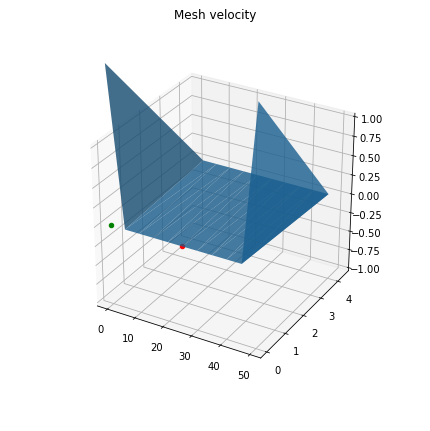
\includegraphics[width=1\linewidth]{fig/1d-sample6}
      \caption{After 6 samples.}
      \label{fig:1d-sample6}
    \end{subfigure}
    \caption{Simulation for a mesh of
    width 52.21 mm, height 2.35 mm, spatial resolution 5 mm.}
    \label{fig:1dcase}
\end{figure}

Perhaps the simplest case of 2D membrane is the degenerate
case of a one-dimensional string. By setting the Y-axis to an
amount that is lower than a full \(\Delta s\) we essentially
obtain this structure. We can excite the structure with a
unit impulse and we obtain the periodic reflection of that impulse
across twelve samples for a 11-point mesh size. The impulse
travels back and forth with no apparent loss of energy
(figure \ref{fig:1dcase}).

\begin{figure}
    \centering
    \begin{subfigure}{.45\textwidth}
      \centering
      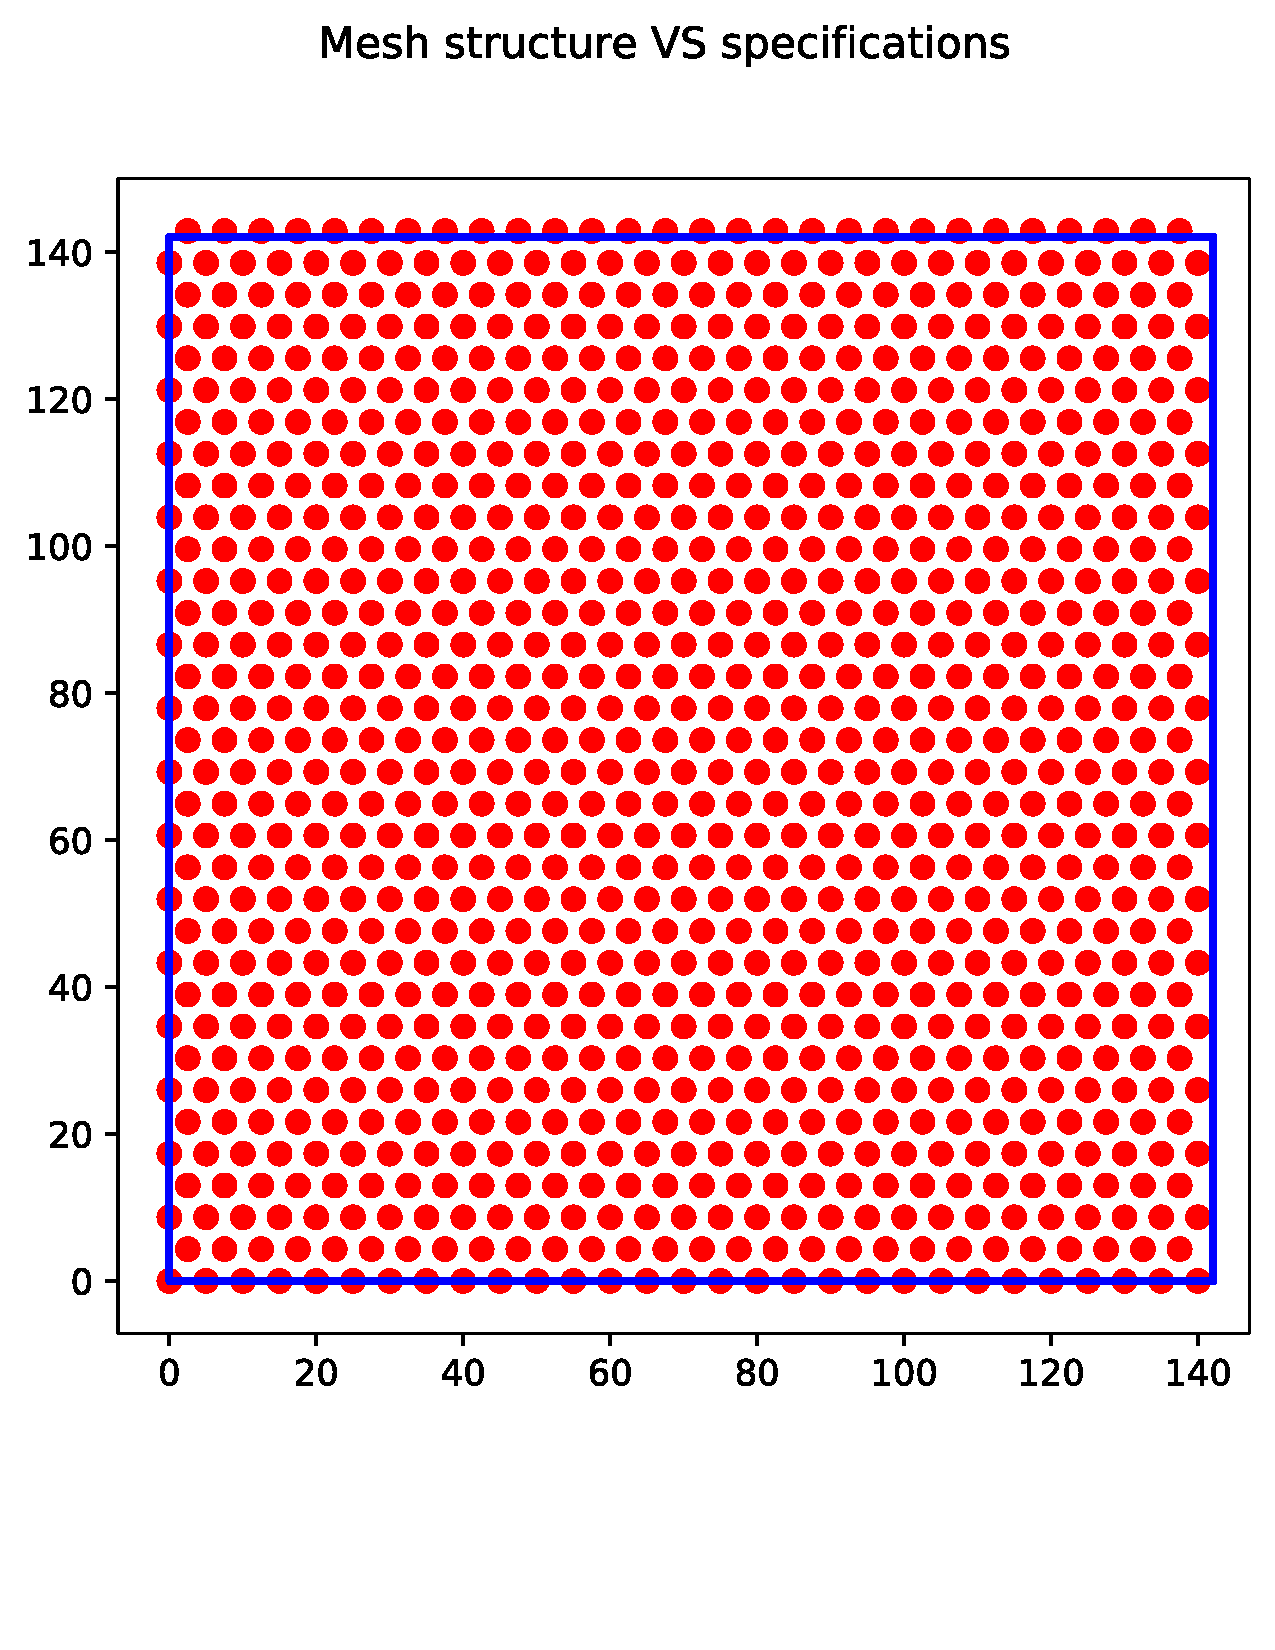
\includegraphics[width=0.8\linewidth]{fig/2d-mesh}
      \caption{Mesh structure.}
      \label{fig:2d-mesh}
    \end{subfigure}%
    \begin{subfigure}{.45\textwidth}
      \centering
      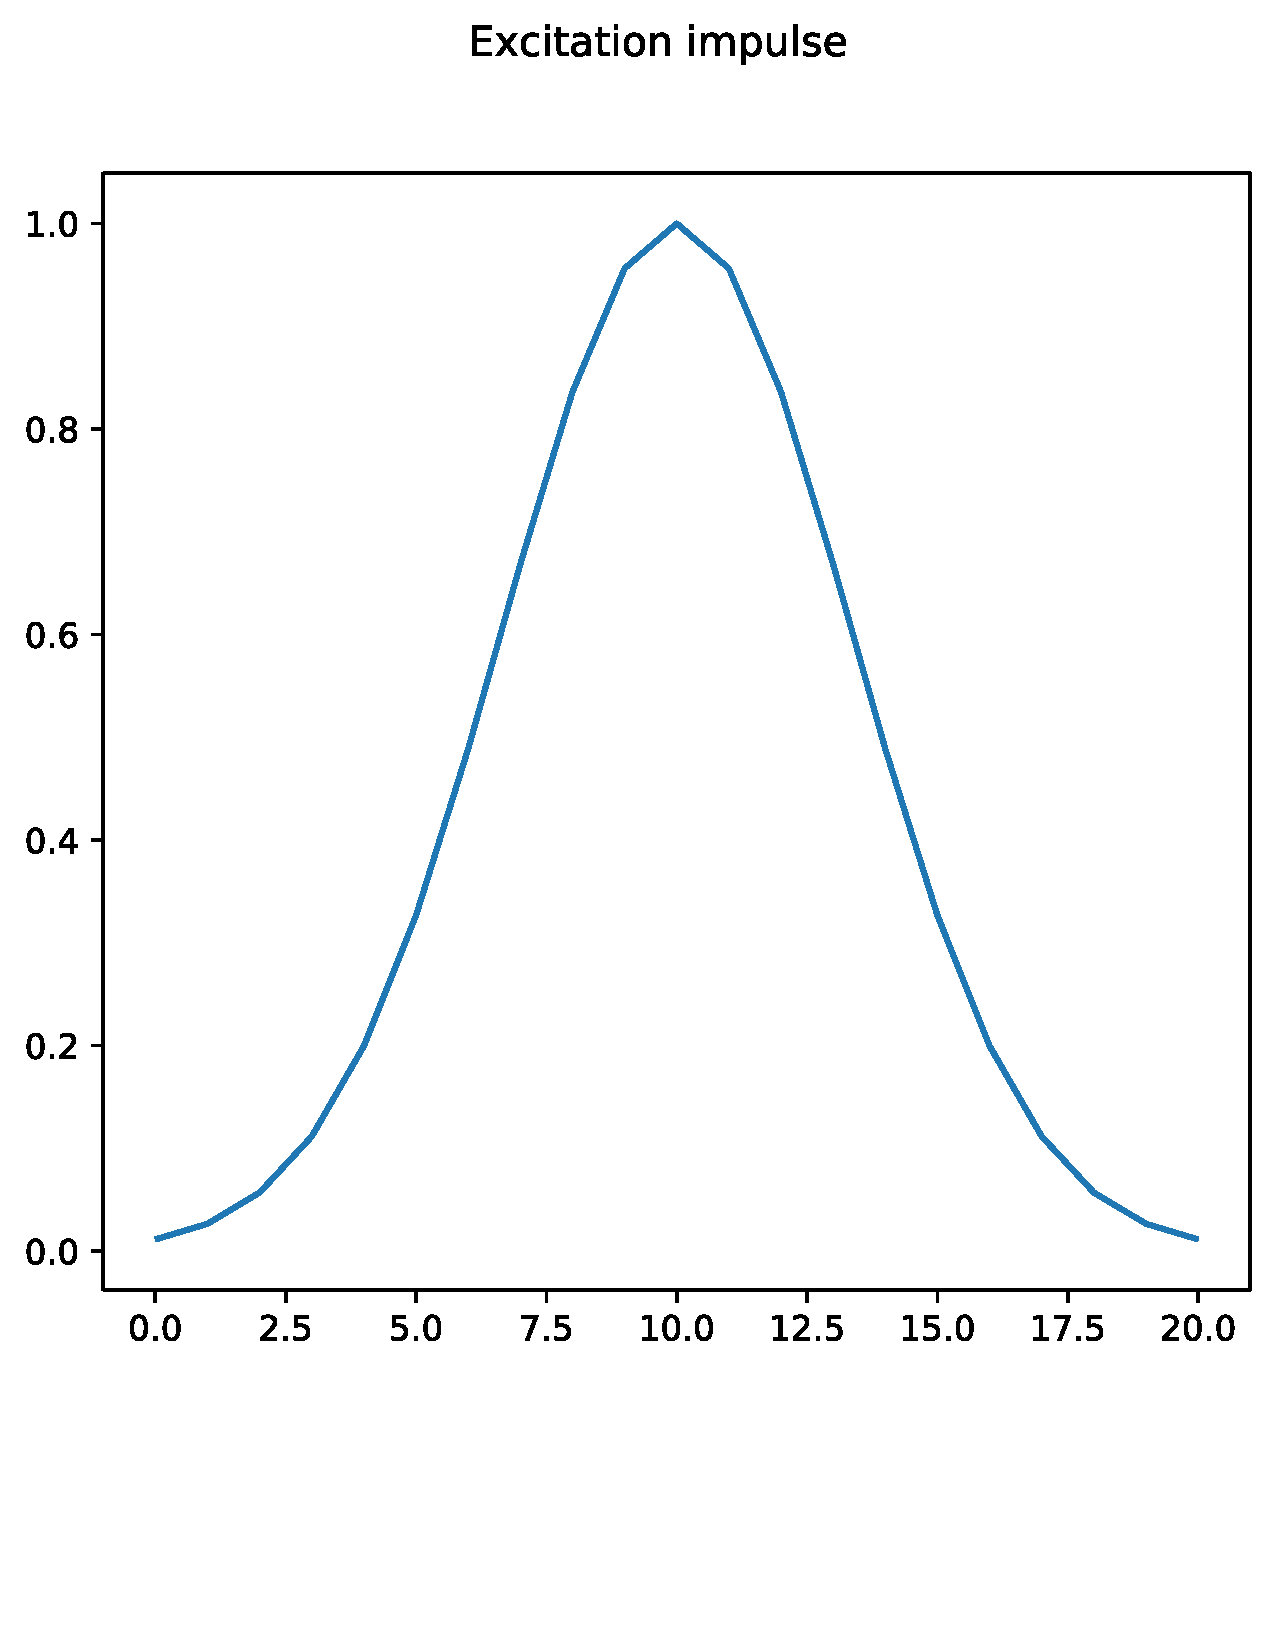
\includegraphics[width=0.8\linewidth]{fig/2d-impulse}
      \caption{Input impulse.}
      \label{fig:2d-impulse}
    \end{subfigure} \\
    \begin{subfigure}{.45\textwidth}
      \centering
      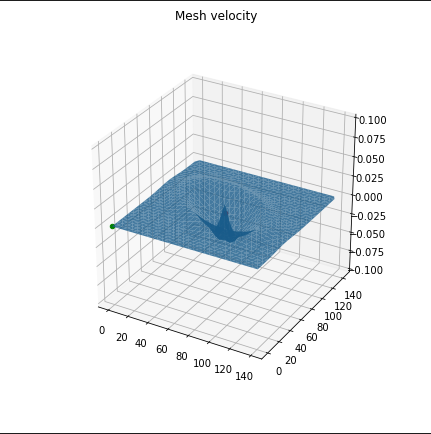
\includegraphics[width=0.8\linewidth]{fig/2d-sample20}
      \caption{Evaluation after 20 samples.}
      \label{fig:2d-sample20}
    \end{subfigure}
    \begin{subfigure}{.45\textwidth}
      \centering
      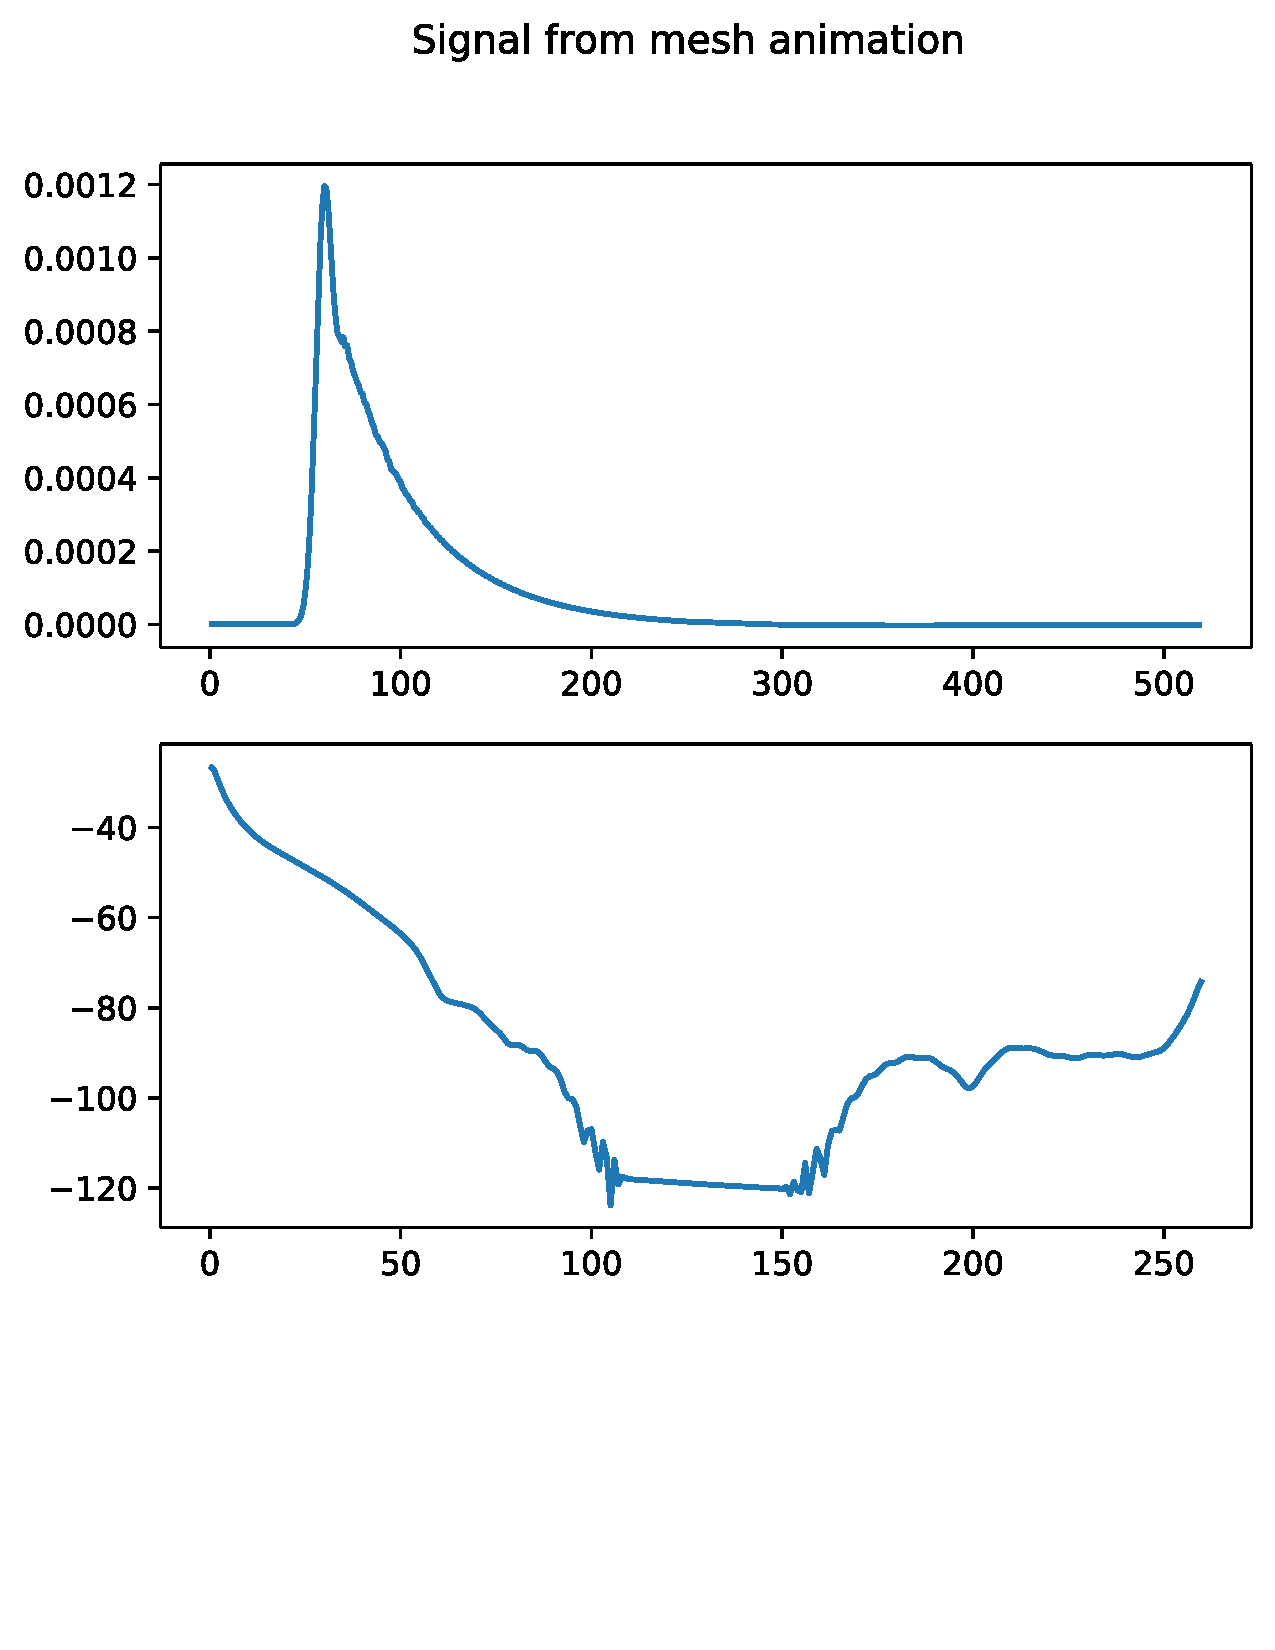
\includegraphics[width=0.8\linewidth]{fig/2d-pickup}
      \caption{Pickup signal in time and frequency (magnitude spectrum).}
      \label{fig:2d-pickup}
    \end{subfigure}
    \caption{Simulation for 142x142 mm mesh, spatial resolution 5 mm.}
    \label{fig:2dcase}
\end{figure}

The next step taken was to simulate a larger rectangular ideal
membrane excited by a Gaussian impulse, with the expectation
that the impulse would propagate radially to the edge
of the membrane and it would scatter at the edges. Figure
\ref{fig:2dcase} outlines the result: the impulse seems to create
a circular shape around the source. The Jupyter animation follows with
what looks like a potentially correct evolution, however
it seems that most of the energy is dissipated really early on
after the event's onset. This is confirmed when examining the pickup
signal in detail \ref{fig:2d-pickup}: the signal recorded is
a thousand times quieter than the source, it decays very rapidly
and the spectrum also shows a certain degree of aliasing.

The mesh has also been simulated with a train of Gaussian
impulses hitting it every second at a sample rate of 44,100 Hz,
which is supported by Bela. The simulation confirms that the
sound of the membrane is anything but interesting! The
processed sound is a noisy, aliased version of the input signal
with no noticeable resonance, and sadly this process has very little
artistic or creative value!

\subsection{On-Target Evaluation}

The specifications of mesh that is suitable for Bela can be
found in the second section of the Jupyter notebook used for the
validation.
Suitable values for \(c\) and the membrane size have been
found by dealing with the tight upper ceiling imposed by Bela's
computational capability: it seems that the current implementation
can only perform the processing of
a 7x6 point mesh at the native sampling rate.

We made a first attempt with a mesh with that number of points,
to verify its stability
when it is controlled by the accelerometer. The system
just shows the very unimpressive feature of boosting
the noise floor of the accelerometer's signal. 

One last attempt was made using the 1-d degenerate case,
which showed a good amount of energy retention. Although the
sonic outcome did not quite improve as much as expected,
the Bela oscilloscope showed a clear modification of the
input waveform, with the impulse being reflected back
and forth and creating a feeble attempt at a standing wave
(figure \ref{fig:bela}).


\begin{figure}
    \centering
    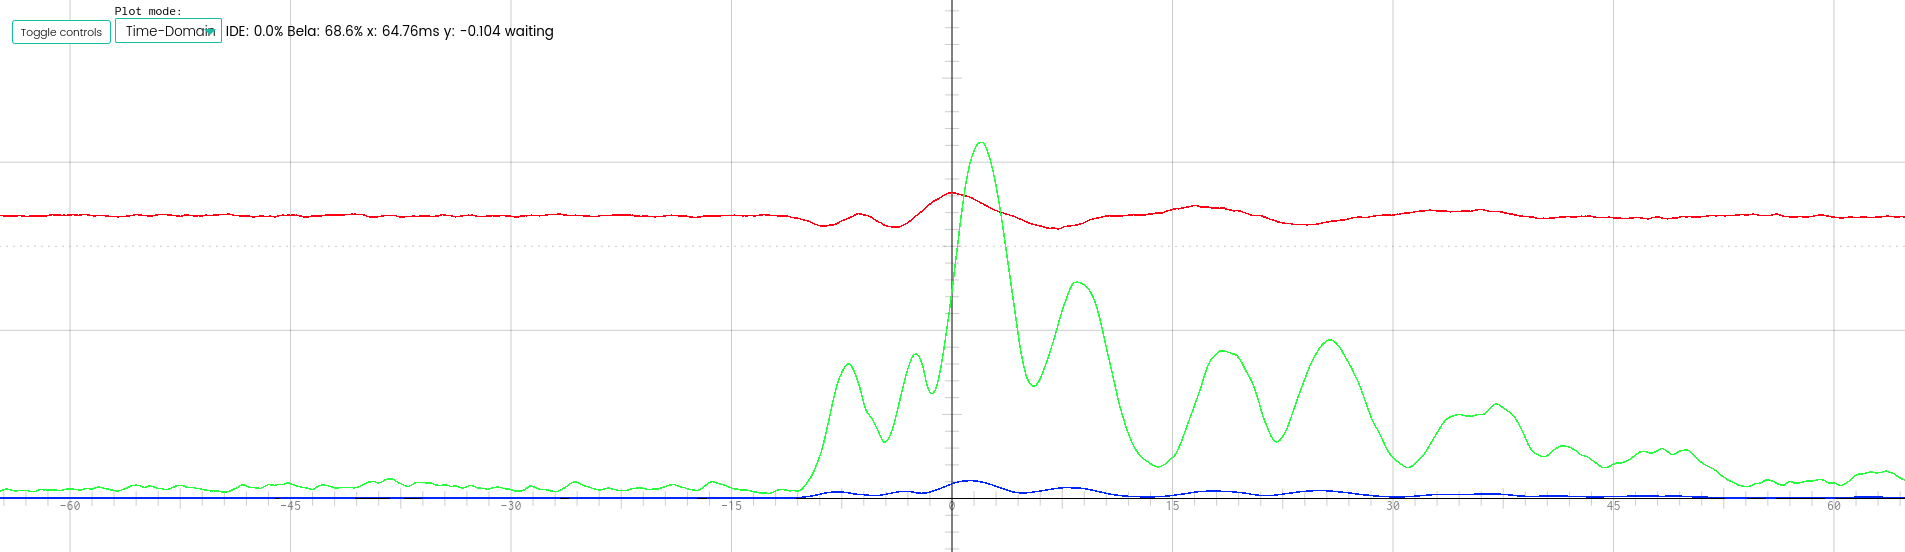
\includegraphics[width=\textwidth]{fig/bela-hit}
    \caption{Representation of a tap from Bela's oscilloscope:
    red line is unfiltered Z-axis signal;
    blue line is filtered signal;
    green line is mesh output.}\label{fig:bela}
\end{figure}


\section{Conclusions and Future Work}

This work has successfully implemented the initial steps
to obtain a fully working implementation of a membrane on Bela.
The task has turned out to be very ambitious and difficult to
correctly achieve within the allocated time frame; however
we managed to run a simple rectangular membrane model in real-time
on Bela that satisfies stability constraints and shows some degree
of physical valitidy in the simulation.

Further work is definitely needed in the understanding of the
relationship between the time sampling rate and the medium speed:
this might be key to achieving more resonating and ``interesting''
membranes, perhaps after implementing multi-rate processing and
oversampling on Bela. In order to progress to this stage,
much work must be done in the mesh's processing function to
use ARM's SIMD intrinsics. The mesh's topology lends itself very
well to vector operations, and ARM chips usually do not
penalise non-contiguous memory accesses.

Furthermore, more in-depth validation is needed to understand
whether the attenuation is a result of the modelling method
or a non-obvious code bug. 1D tests could be run along \(l\)--
and \(m\)--axis to verify that impulse propagation happens
correctly in all directions. Modal analysis, including mode shifting
as a result of attenuation, is also a common method to validate
the physics of a membrane model \cite{fontana1998physical}.
After reaching this stage, attenuation coefficients and air
loading can be implemented and correctly validated.

\begin{thebibliography}{9}

\bibitem[Rossing, 2004]{rossing2004acoustics}
Rossing, T.D., Yoo, J. and Morrison, A., 2004.
\textit{Acoustics of percussion instruments: An update.}
Acoustical science and technology, 25(6), pp.406-412.

\bibitem[Bilbao, 2009]{bilbao2009modular}
Bilbao, S., 2009, September.
\textit{A modular percussion synthesis environment.}
In Proc. of the 12th Int.
Conference on Digital Audio Effects (DAFx-09), Como, Italy.

\bibitem[Mehes, 2017]{mehes2017virtual}
Mehes, S., van Walstijn, M. and Stapleton, P., 2017.
\textit{Virtual-acoustic instrument design:
exploring the parameter space of a string-plate model.}
In NIME (pp. 399-403).

\bibitem[Fontana, 1998]{fontana1998physical}
Fontana, F. and Rocchesso, D., 1998.
\textit{Physical modeling of membranes for percussion instruments.}
Acta Acustica united with Acustica, 84(3), pp.529-542.

\bibitem[Murphy, 2000]{murphy2000digital}
Murphy, Damian Thomas, and D. M. Howard.
\textit{Digital waveguide mesh topologies in room acoustics modelling.}
Diss. University of York, 2000.

\bibitem[Baldan, 2017]{baldan2017sound}
Baldan, S., Delle Monache, S. and Rocchesso, D., 2017.
\textit{The Sound Design Toolkit.} SoftwareX, 6, pp.255-260.

\bibitem[Trautmann, 2001]{trautmann2001physical}
Trautmann, L., Petrausch, S. and Rabenstein, R., 2001, May.
\textit{Physical modeling of drums by transfer function methods.}
In 2001 IEEE International Conference on Acoustics,
Speech, and Signal Processing. Proceedings
(Cat. No. 01CH37221) (Vol. 5, pp. 3385-3388). IEEE.

\bibitem[Laird, 2001]{laird2001physical}
Laird, J.A., 2001.
\textit{The physical modelling of drums using digital waveguides.}
(Doctoral dissertation, University of Bristol).

\end{thebibliography}


\end{document}